\chapter{Técnicas de Monitoreo Estructural}

\section{Motivación}

Nunca se está seguro de las propiedades \emph{exactas} de una estructura. 

\begin{enumerate}
    \item Obras civiles ``envejecen'':
    \begin{itemize}
        \item Daño/deterioro estructura $\longrightarrow$ Cambio en las propiedades de materiales
    \end{itemize}
    \item Incertidumbre:
    \begin{itemize}
        \item Propiedades nominales utilizadas en diseño
        \item Los modelos nominales no necesariamente representan fielmente el comportamiento real de la estructura
    \end{itemize}
\end{enumerate}

Un buen proyecto de monitoreo estructural (Structural health monitoring, SHM) tiene múltiples objetivos más allá de la instrumentación.

\begin{figure}[H]
    \centering
    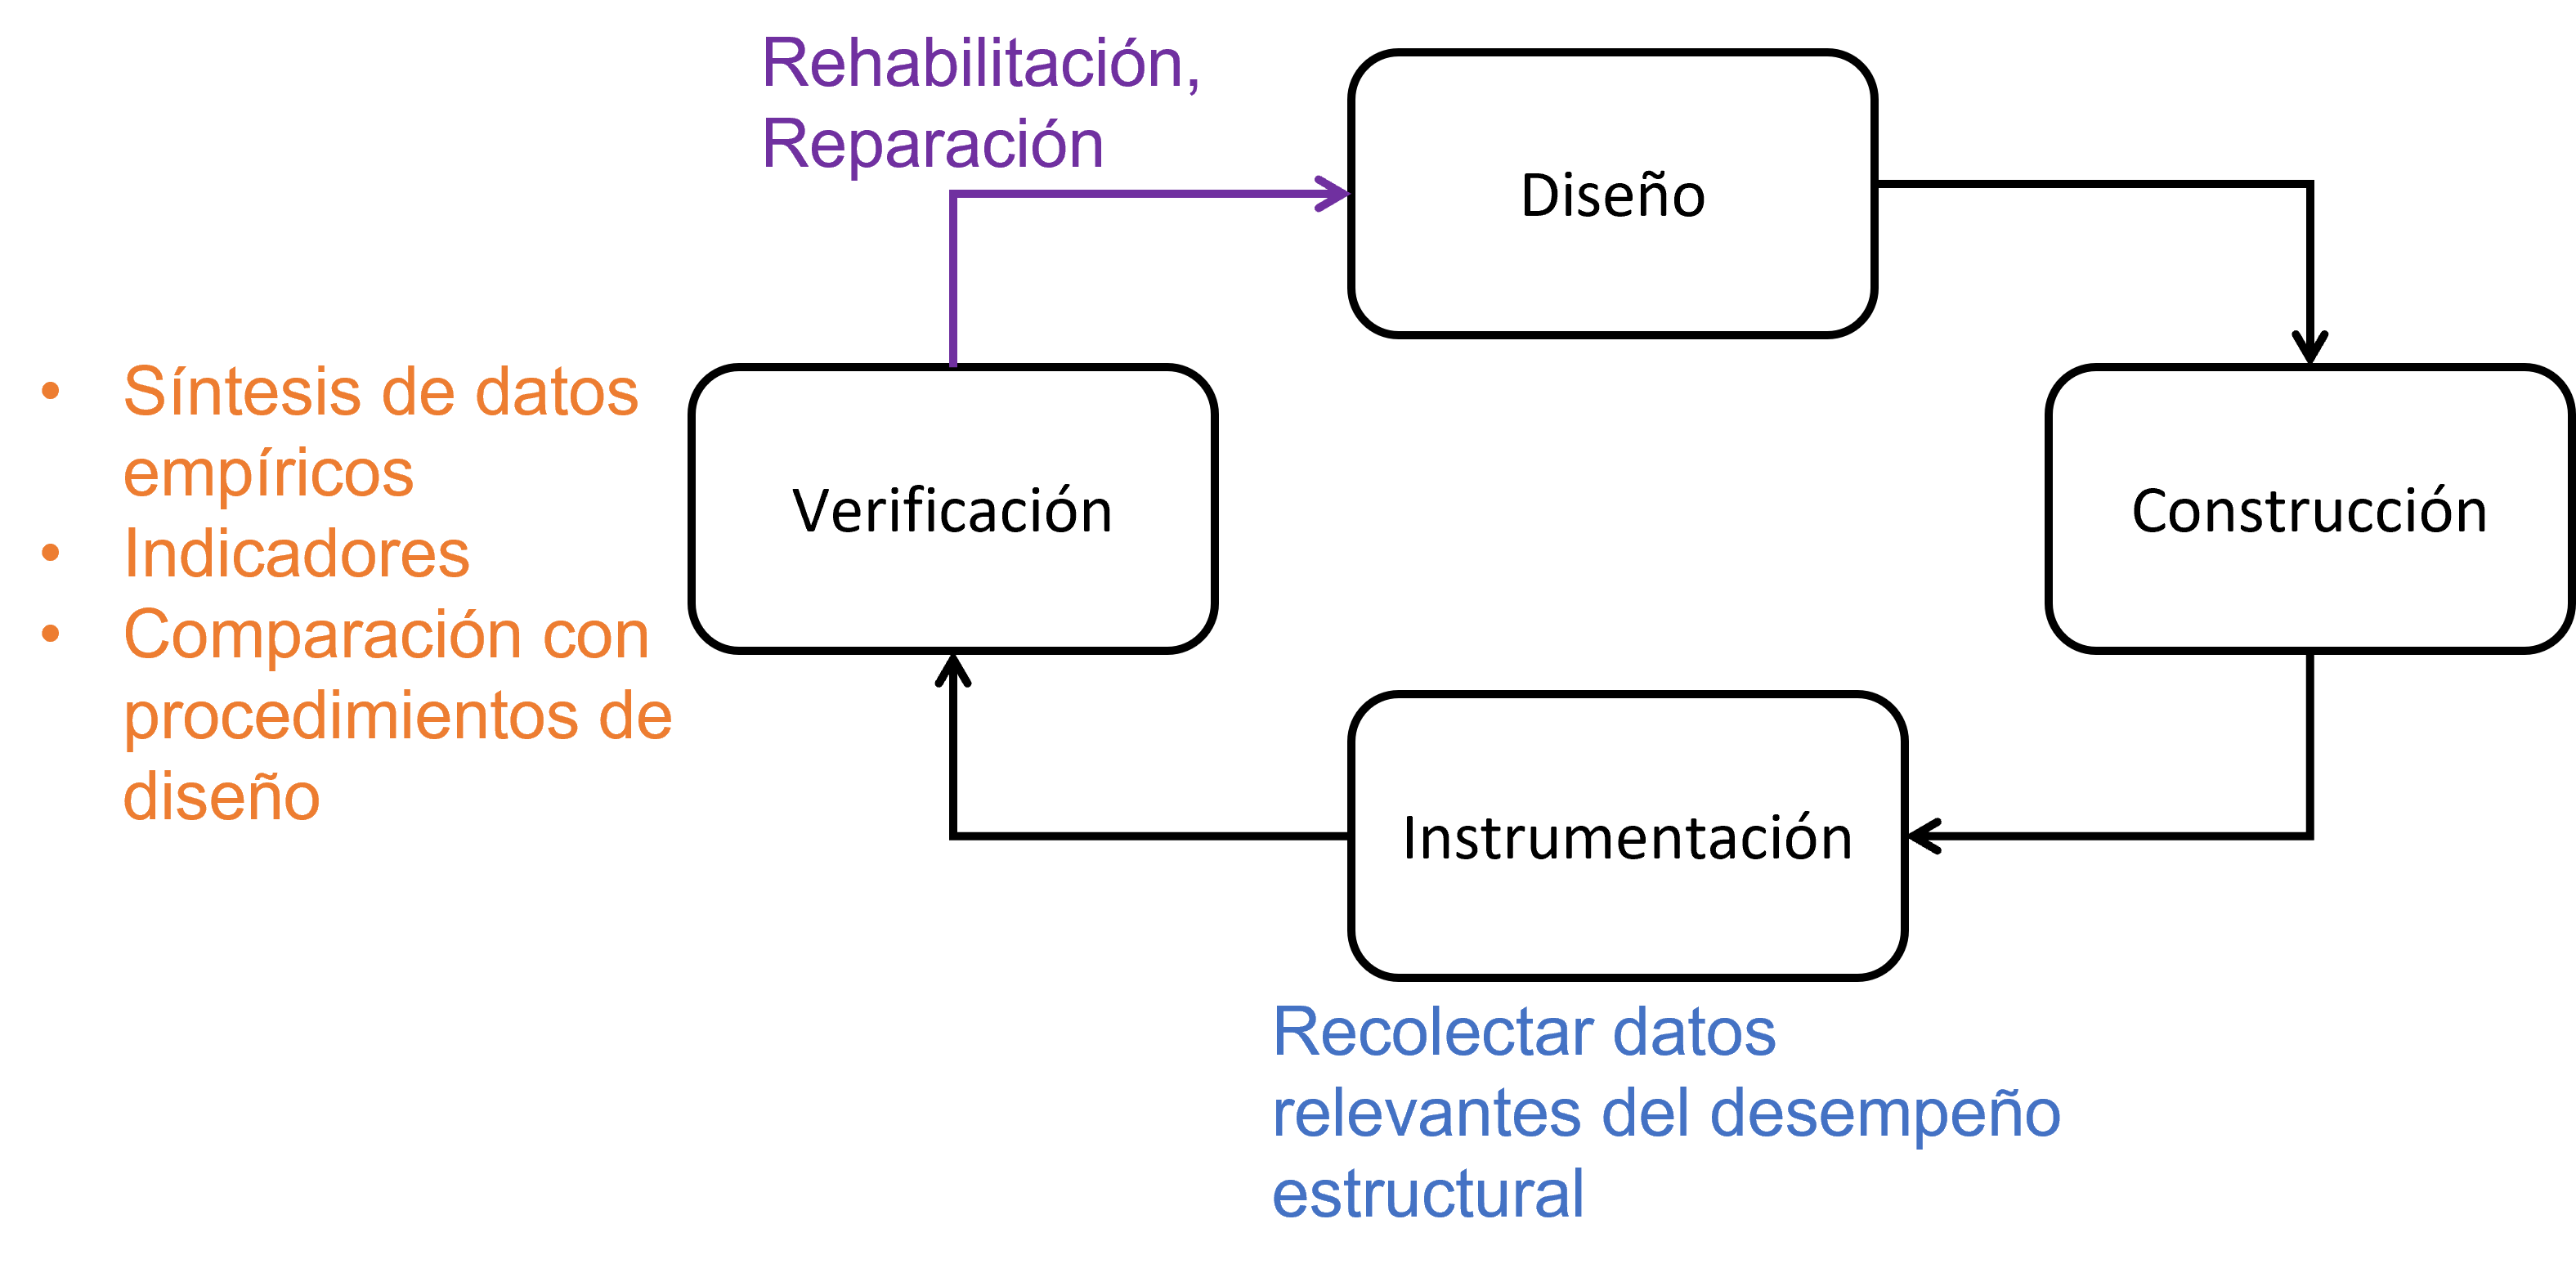
\includegraphics[scale=0.5]{Figuras/sysID.png}
\end{figure}

Para el monitoreo estructural se busca:

\begin{itemize}
    \item Determinar un modelo matemático de un sistema.
    \item Realizar predecicción: desempeño, daño,
\end{itemize}

\section{Identificación de Sistemas}

\subsection{Generalidades}

\begin{enumerate}
    \item Análisis dinámico (problema directo)
    \begin{figure}[H]
    \centering
    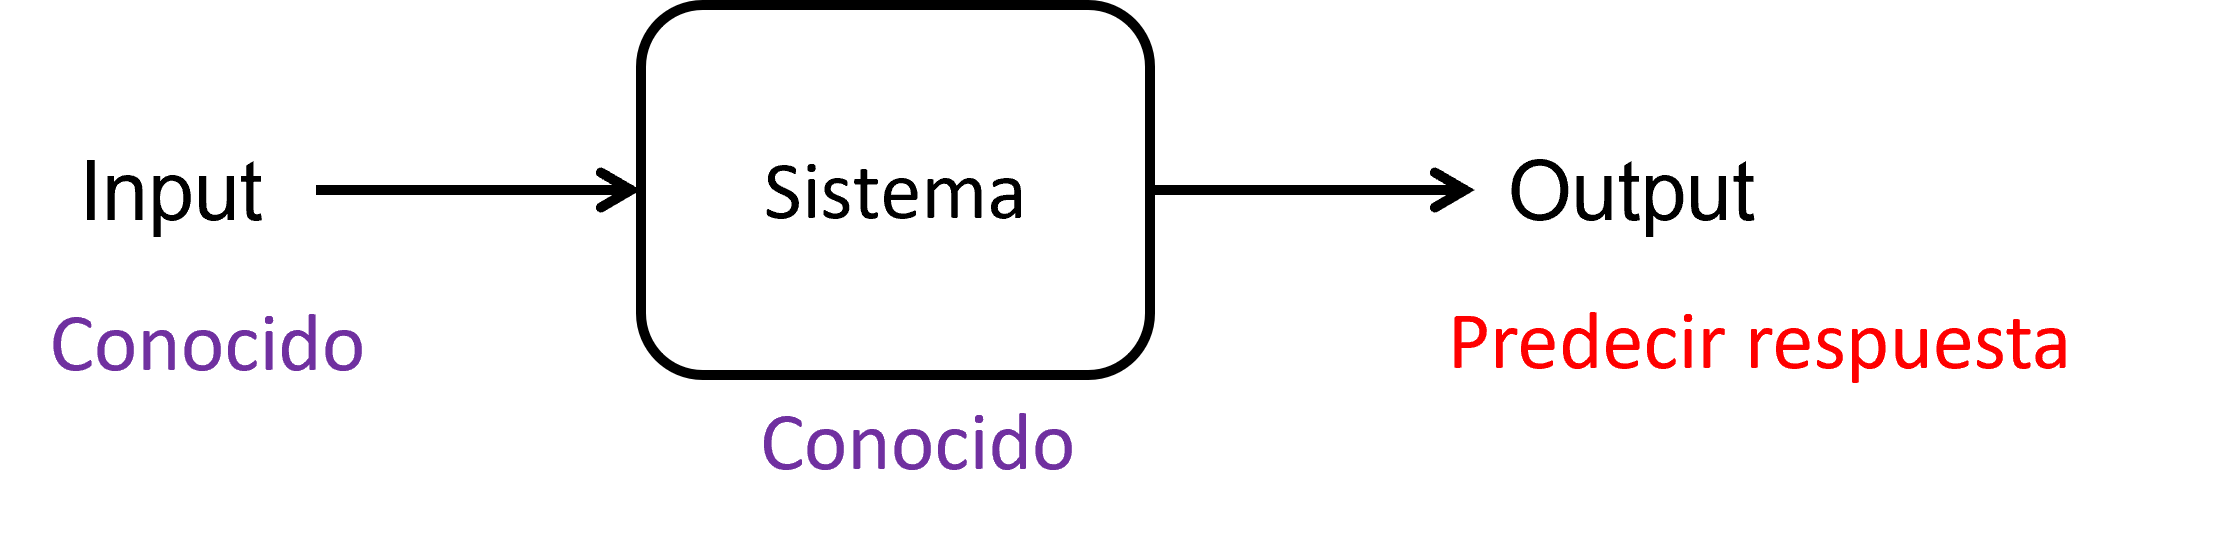
\includegraphics[scale=0.6]{Figuras/problema_directo.png}
    \end{figure}
    \item Identificación de fuerza de entrada
    \begin{figure}[H]
    \centering
    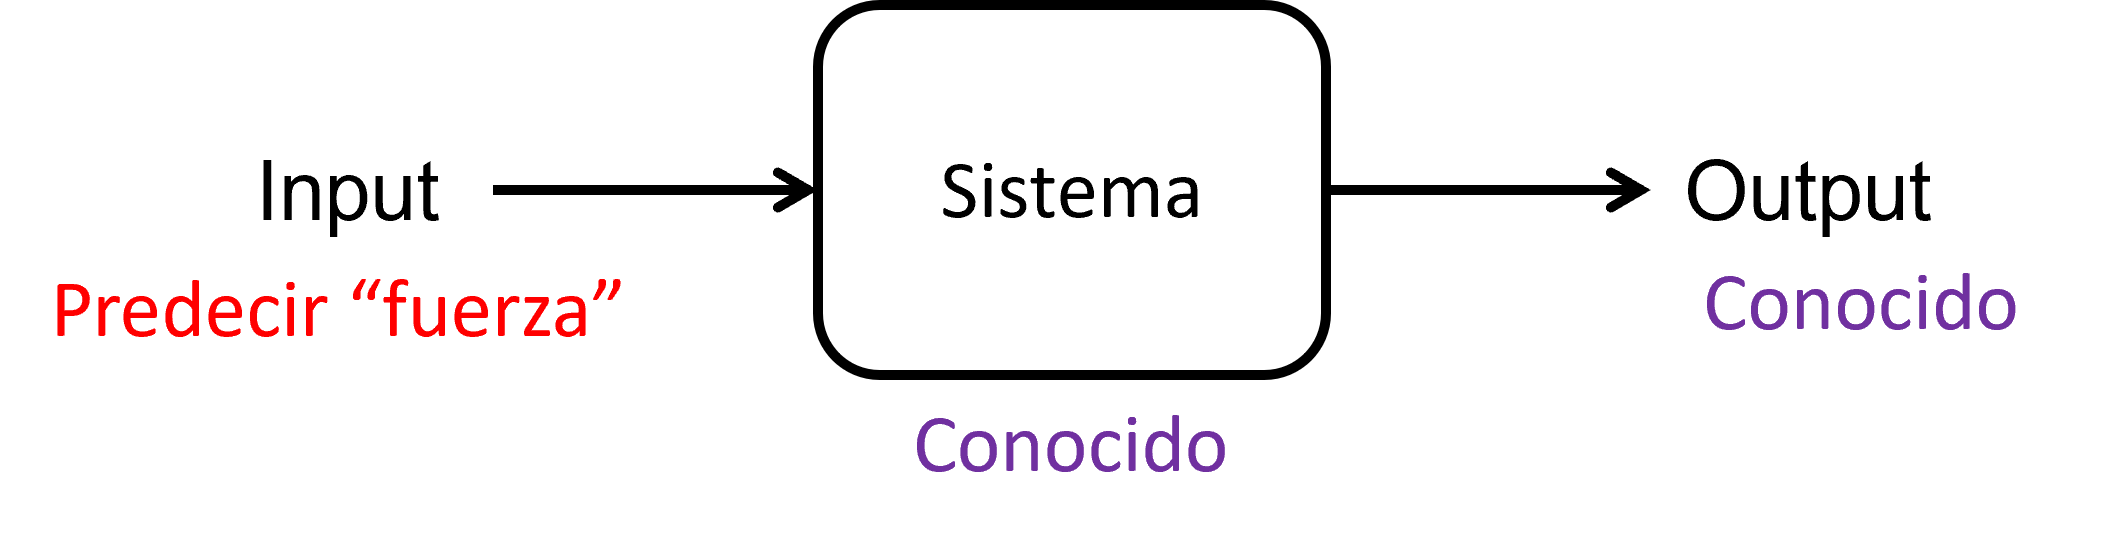
\includegraphics[scale=0.6]{Figuras/fuerza_entrada.png}
    \end{figure}    
    \item Identificación de sistema
    \begin{figure}[H]
    \centering
    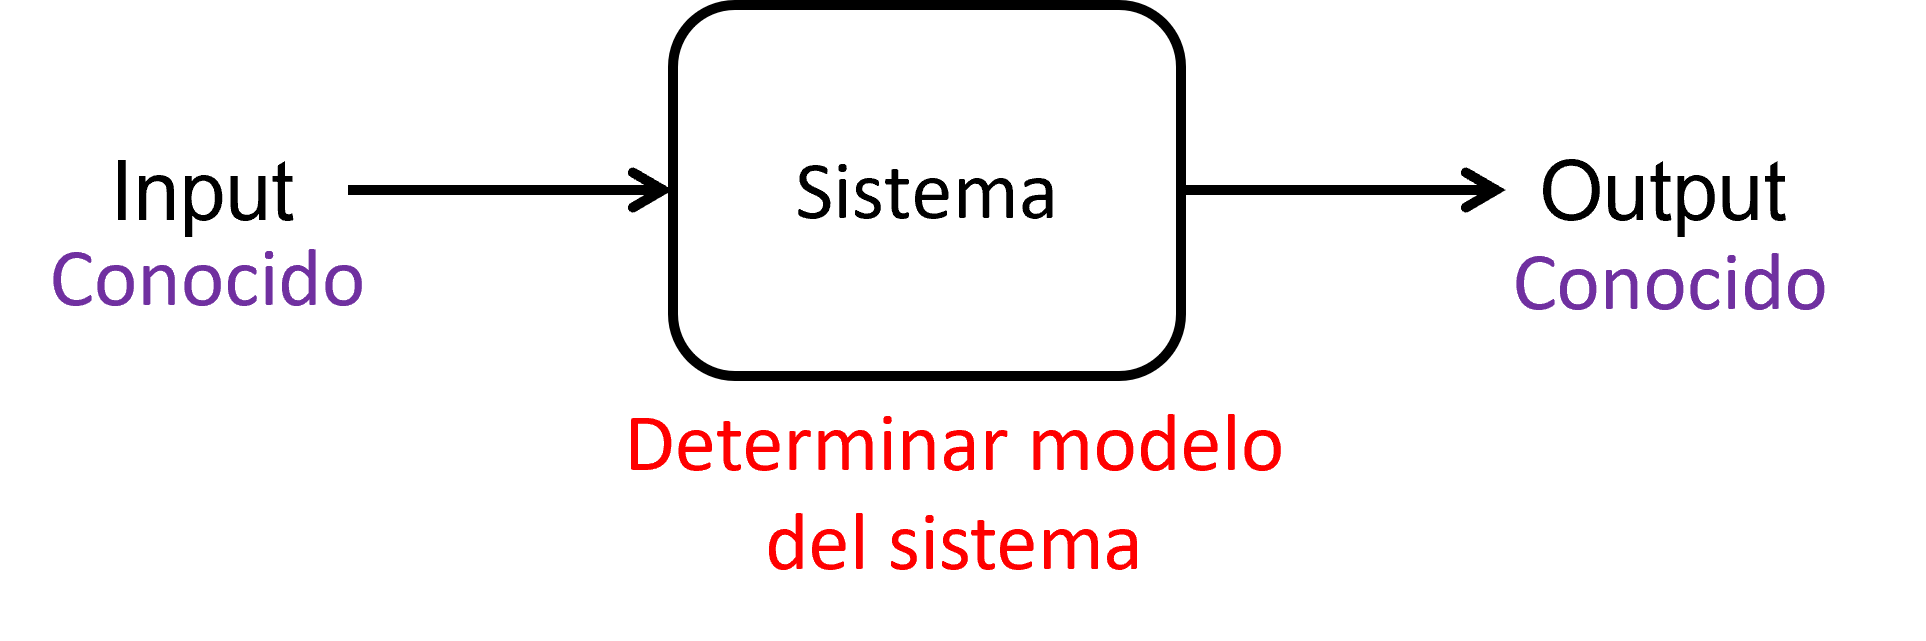
\includegraphics[scale=0.6]{Figuras/problema_inverso.png}
    \end{figure}
\end{enumerate}

Estas predicciones se pueden realizar con distintos métodos:

\begin{enumerate}
    \item Basados en dominio frecuencia
    \begin{itemize}
        \item Análisis modal experimental
        \item Optimización no paramétrica
    \end{itemize}
    \item Basados en dominio tiempo
    \begin{itemize}
        \item Modelos auto-regresivos: ARX, ARMA, ARMAX, etc.
        \item Métodos basados en subespacios: ERA, Next-ERA, SSI, etc.
    \end{itemize}
\end{enumerate}

Resumen de identificación de sistemas (SysID):

\begin{figure}[H]
    \centering
    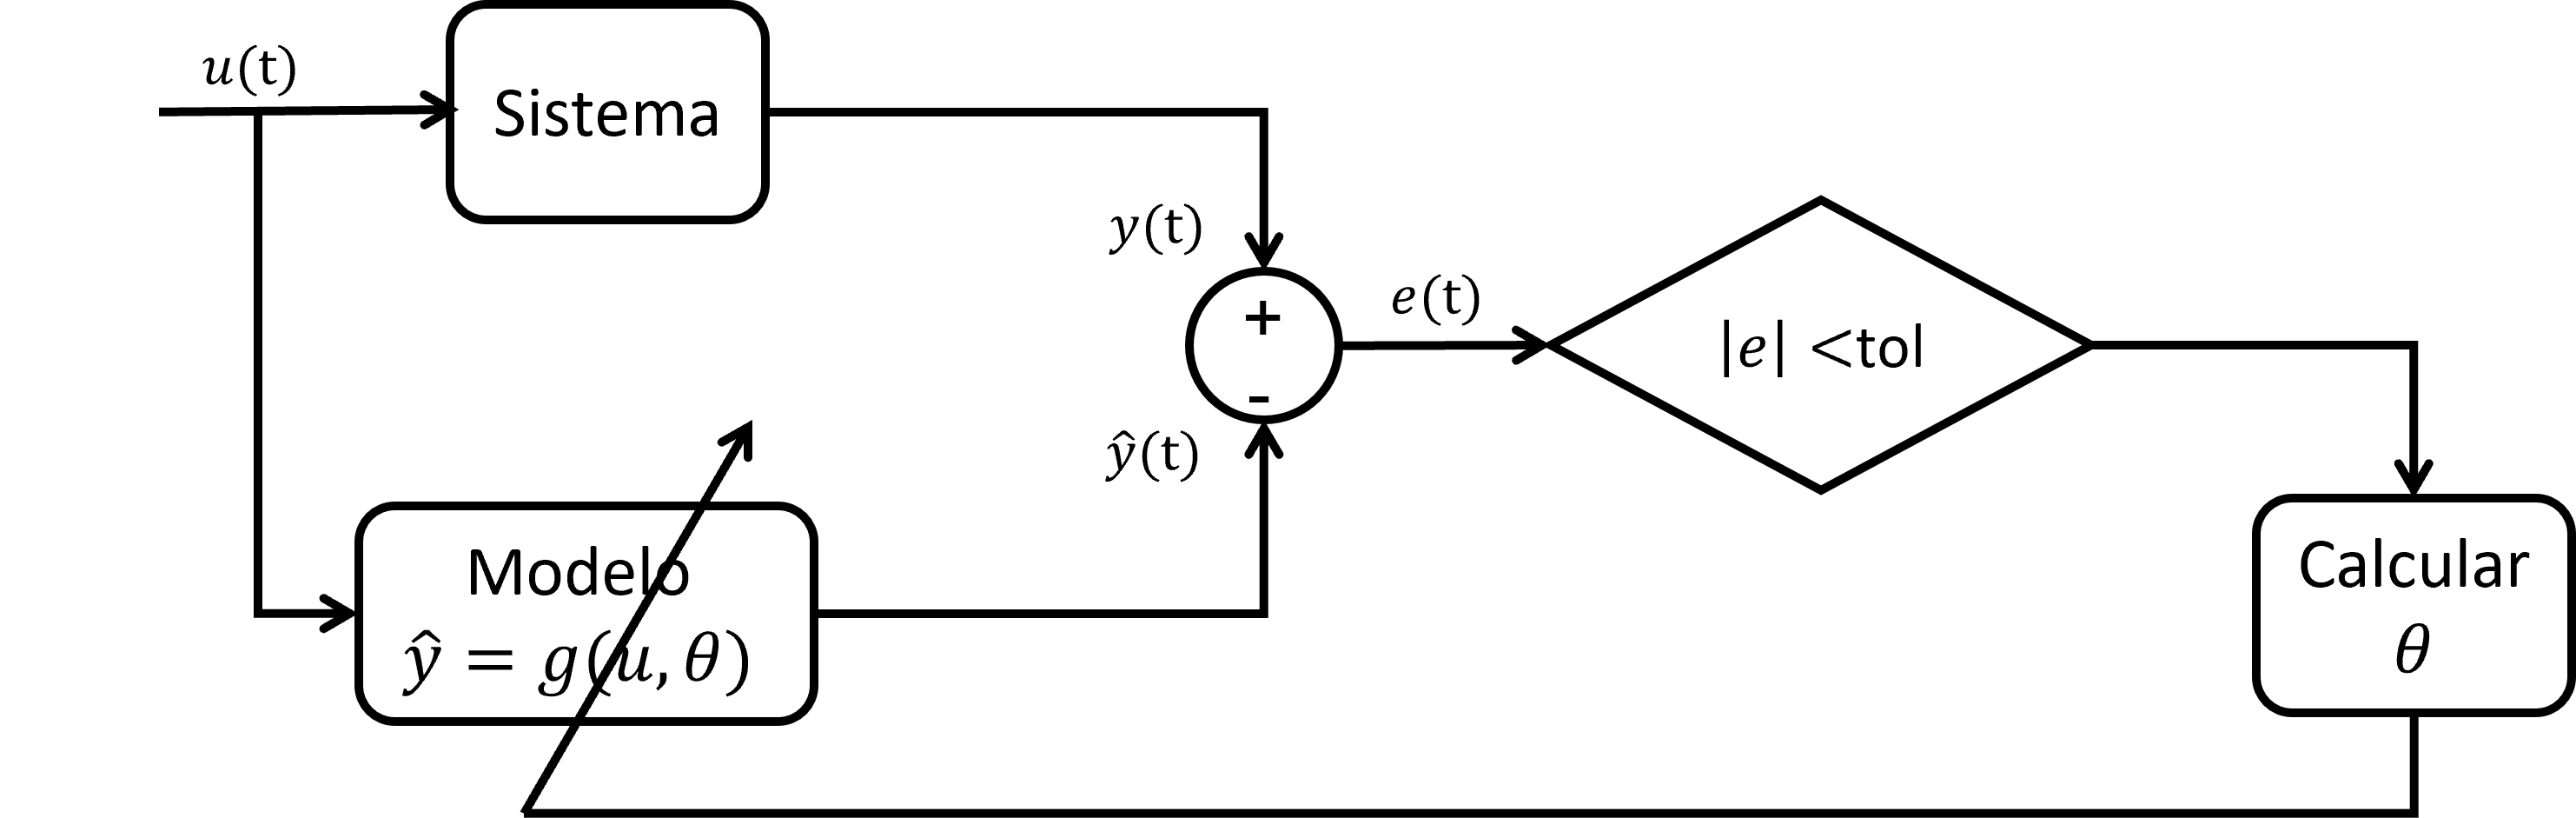
\includegraphics[width=5in]{Figuras/resumenSysID.png}
\end{figure}

\section{Métodos no-paramétricos de estimación espectral}

Referencias: \textcite[Sec. 18.4]{craig2006fundamentalsstructural} y \textcite[Cap. 6]{Bendat2011}. 

\subsection{Definiciones}

Dado un sistema LTI con entrada $u(t)$ y salida $y(t)$ conocidos experimentalmente, buscamos determinar de forma estimada su FRF, $G_{YU}(\omega)$.\\

\begin{figure}[H]
    \centering
    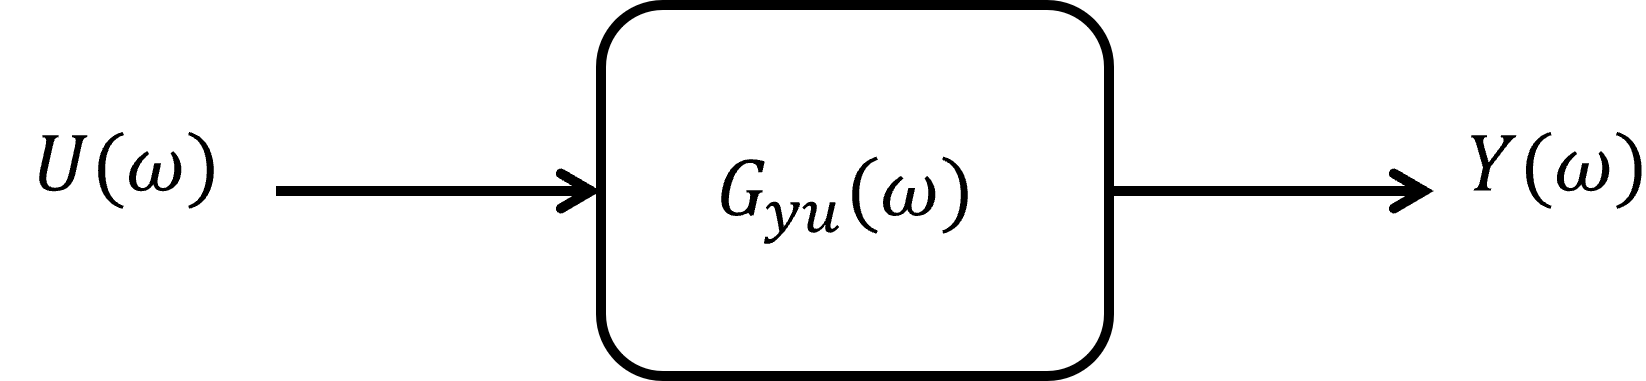
\includegraphics[scale=0.6]{Figuras/UY.png}
\end{figure}

\begin{align*}
    Y(\omega) &= G_{YU}(\omega)U(\omega) \quad \text{(FRF)}\\
    y(t) &= (g_{YU} \ast u)(t) \quad \text{(FRI)}
\end{align*}

Nota: Relación entre FRF y FRI: $G_{YU}(\omega) = \mathcal{F}\{g_{YU}(t)\}$

\subsection{Densidad de poder espectral finita}

\par Recordando el teorema de Wiener-Khinchin, que establece la relación entre \emph{densidad de poder espectral} ($S_{XX}(\Omega)$) y \emph{autocorrelación} ($R_{XX}(\tau)$) de un proceso estocástico w.s.s. $\{X(t),t \in T\}$:

\begin{align*}
    S_{XX}(\Omega) &= \mathcal{F}\{R_{XX}(\tau)\}\\
    R_{XX}(\tau) &= \mathcal{F}^{-1}\{S_{XX}(\Omega)\}
\end{align*}

\noindent donde $R_{XX}(\tau) =\mathbb{E}\{X(t)X(t+\tau)\}$ y $\mathcal{F}\{\cdot\}$ es la transformada de Fourier (contínua).\\

% Ver PSD finito. \parencite[Cap. 5]{Bendat2011}

Mientras, para el caso en tiempo discreto se utiliza la definición de \emph{periodograma}. Suponiendo una muestra finita de $N$ puntos del p.e. $\{X(t),t \in T\}$, con período de muestreo $T_s$:

\begin{align*}
    x[n] =
    \begin{cases}
        x(n T_s), & n\in\{0,1,\ldots,N-1\}\\
        0, & \text{otherwe}
    \end{cases}
\end{align*}

Entonces, el \emph{periodograma} se define como: 

\begin{align*}
    \hat{S}_{XX}(\omega) = \frac{1}{N} X(\omega) X(\omega)^{*} = \frac{1}{N} |X(\omega)|^{2}
\end{align*}

\noindent donde $X(\omega)$ es la transformada de Fourier de tiempo discreto (DTFT) de la señal finita $x[n]$:

\begin{align*}
    X(\omega) = \sum_{n=0}^{N-1} x[n] e^{-j \omega n}
\end{align*}

\noindent y $(\cdot)^{*}$ es la transpuesta conjugada.\\

\emph{Nota:} $S_{XX}(\omega)$ es un valor real.\\

En el límite para $N\to\infty$, el periodograma (un estimador sesgado del PSD) converge al valor real del PSD:

\begin{align*}
    S_{XX}(\omega) = \lim_{N\to\infty} \mathbb{E} \left\{ \hat{S}_{XX}(\omega) \right\}
\end{align*}

Para todo el estudio que viene a continuación consideramos estimaciones de PSD utilizando alguna de las definiciones de periodograma modificado (por ejemplo, método de Welch). %, y para simplificar la notación, utilizaremos ${S}_{XX}(\omega)$ (sin sombrero) como para referirnos a la estimación del PSD de $x(t)$.

\subsection{Relaciones entrada-salida de poder espectral}

Asumir que $u(t)$ e $y(t)$, entrada y salida de un sistema LTI SISO determinístico, son procesos estocásticos w.s.s. de media cero. Entonces, calculemos un estimador del auto PSD de la respuesta $y(t)$:

\begin{align*}
    \hat{S}_{YY}(\omega) &= \frac{1}{N} Y(\omega)Y^{*} (\omega)\\\
    &= \frac{1}{N} \left( G_{YU}(\omega) U(\omega)\right) \left(G_{YU}(\omega) U(\omega)\right)^{*}\\
    &= \frac{1}{N} G_{YU}(\omega) U(\omega) U(\omega)^{*} G_{YU}(\omega)^{*}
\end{align*}

Si el sistema es determinístico, con parámetros sin incertidumbre pero desconocidos:

\begin{align*}
    \hat{S}_{YY}(\omega) &= G_{YU}(\omega) G_{YU}(\omega)^{*} \underbrace{\left\{ \frac{1}{N}U(\omega) U(\omega)^{*} \right\}}_{_{\hat{S}_{UU}(\omega)}}\\
    \hat{S}_{YY}(\omega) &= \left| G_{YU}(\omega) \right|^2 \hat{S}_{UU}(\omega)\\
    \left| G_{YU}(\omega) \right|^2 &= \frac{\hat{S}_{YY}(\omega)}{\hat{S}_{UU}(\omega)}
\end{align*}

\underline{Nota}: $|G_{YU}(\omega)|^2$ es una función real y nos entrega sólo información de la magnitud del sistema y no de la fase. Por lo tanto, \underline{este método queda descartado}.

\subsection{Método \texorpdfstring{$H_1$}{H1}}

Continuando el estudio del sistema SISO LTI:

\begin{align*}
    Y(\omega) &= G_{YU}(\omega)U(\omega) \quad / \cdot U^{*}(\omega)\\
    Y(\omega)U^{*}(\omega) &= G_{YU}(\omega)U(\omega)U^{*}(\omega) \quad / \frac{1}{N} \cdot \\
    \underbrace{\left\{\frac{1}{N}Y(\omega)U^{*}(\omega)\right\}}_{\hat{S}_{YU}(\omega)} &= G_{YU}(\omega)  \underbrace{\left\{\frac{1}{N} U(\omega)U^{*}(\omega) \right\}}_{\hat{S}_{UU}(\omega)} \\
    \hat{S}_{YU}(\omega) &= G_{YU}(\omega) \hat{S}_{UU}(\omega)\\
    \hat{G}_{YU}(\omega) &= \frac{\hat{S}_{YU}(\omega)}{\hat{S}_{UU}(\omega)} \quad \text{(Estimador $H_1$)}
\end{align*}

donde $\hat{S}_{YU}(\omega)$ es la estimación del PSD cruzado entre respuesta $y(t)$ y entrada $u(t)$.\\

\emph{Nota 1:} $\hat{S}_{YU}(\omega)$ es un número complejo.

\emph{Nota 2:} $\hat{G}_{YU}(\omega)$ es un número complejo. Por lo tanto, este método arroja una estimación de la magnitud  $|\hat{G}_{YU}(\omega)|$ y fase $\angle G_{YU}(\omega)$ del sistema dinámico.

\subsection{Método \texorpdfstring{$H_2$}{H2}}

Otra alternativa es el método $H_2$:

\begin{align*}
    Y(\omega) &= G_{YU}(\omega)U(\omega) \quad / \cdot Y^{*}(\omega)\\
    Y(\omega) Y^{*}(\omega) &= G_{YU}(\omega )U(\omega) Y^{*}(\omega) \quad / \frac{1}{N} \cdot \\
    \underbrace{\left\{\frac{1}{N}Y(\omega)Y^{*}(\omega)\right\}}_{\hat{S}_{YY}(\omega)} &= G_{YU}(\omega)  \underbrace{\left\{\frac{1}{N} Y(\omega)U^{*}(\omega) \right\}}_{\hat{S}_{YU}(\omega)} \\
    \hat{S}_{YY}(\omega) &= G_{YU}(\omega) \hat{S}_{YU}(\omega)\\
    \hat{G}_{YU}(\omega) &= \frac{\hat{S}_{YY}(\omega)}{\hat{S}_{YU}(\omega)} \quad \text{(Estimador $H_2$)}
\end{align*}

\subsection{Método \texorpdfstring{$H_v$}{Hv}}

Otra alternativa es el método $H_v$:

\begin{equation*}
    H_v(\omega) =\Re\{H_v(\omega)\} + j\Im\{H_v(\omega)\}
\end{equation*}

que consiste en la media geométrica de estimadores $H_1$ y $H_2$. En este sentido, la media geométrica se toma para cada parte real e imaginaria del FRF por separado:

\begin{align*}
    \Re\{H_v(\omega)\} & = \sqrt{\Re\{H_1(\omega)\} \Re\{H_2(\omega)\}} \\
    \Im\{H_v(\omega)\} & = \sqrt{\Im\{H_1(\omega)\} \Im\{H_2(\omega)\}}
\end{align*}

\subsection{Mediciones con ruido}

% URL: https://dsp.stackexchange.com/questions/71811/understanding-the-h1-and-h2-estimators

En ausencia de ruido en $u(t)$ y $y(t)$, ambos estimadores $H_1$ y $H_2$ coinciden (caso ideal). Pero, en la situación con ruido en las mediciones de entrada y/o salida, hay diferencias relevantes a considerar.

\begin{figure}[H]
    \centering
    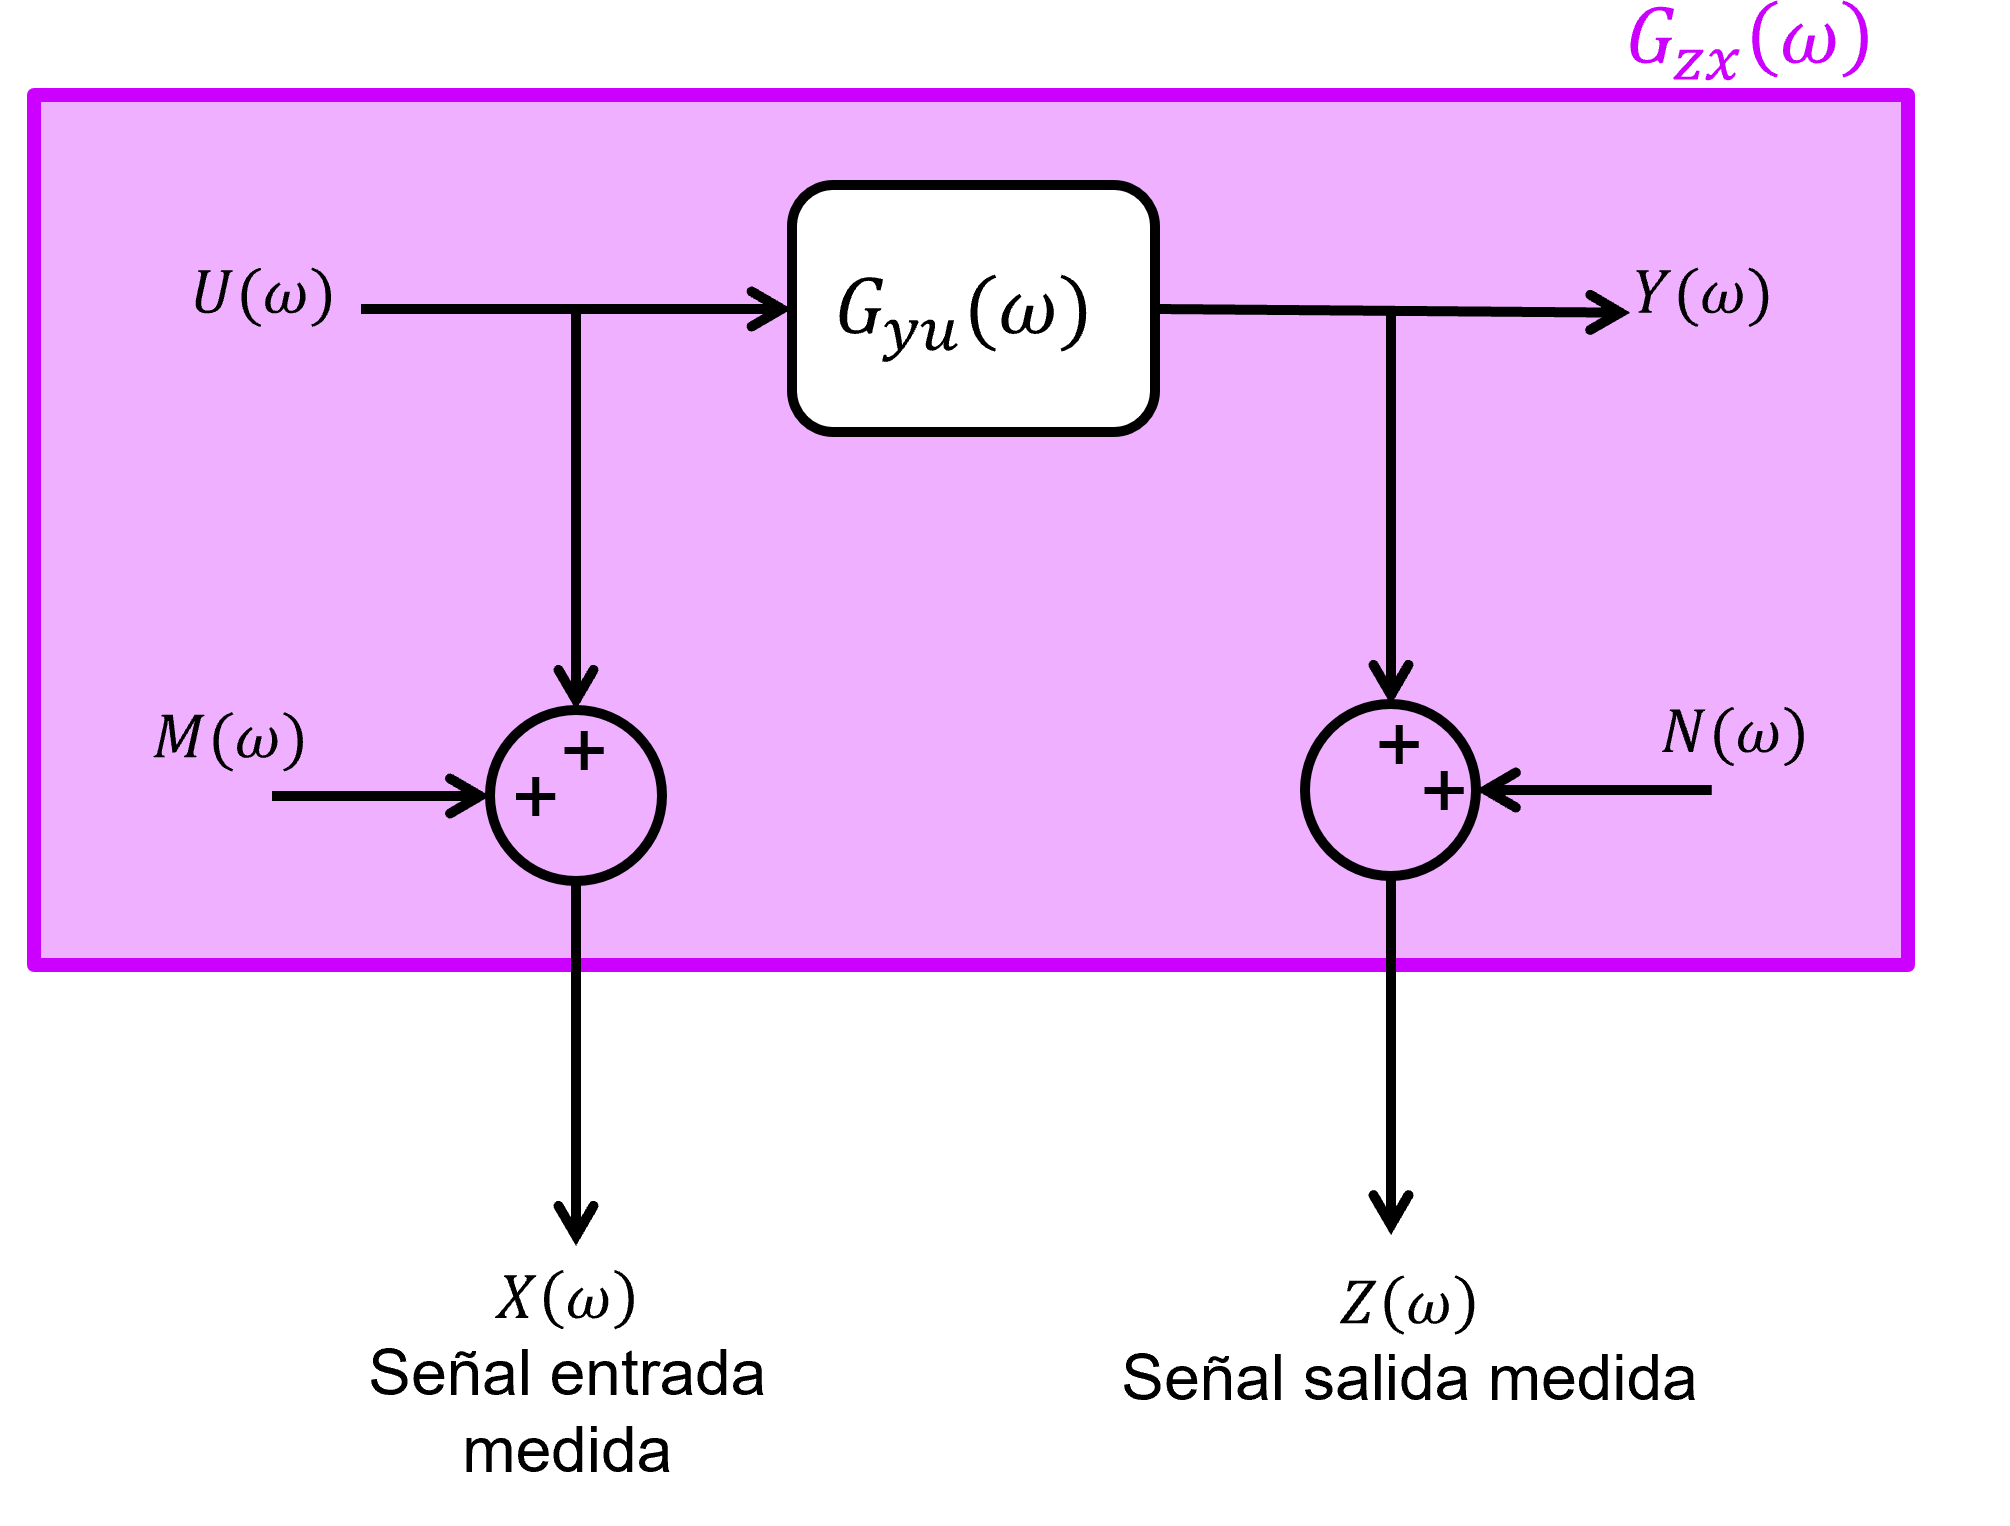
\includegraphics[scale=0.7]{Figuras/H1_ruido.png}
\end{figure}

\par \underline{Nota}: 

\begin{itemize}
    \item Ruido $m(t)$ y $n(t)$ son p.e. estacionarios no correlacionados $\Longrightarrow R_{MN}(\tau) = \mathbb{E}\{m(t) u(t+\tau)\}=0$
    \item Ruido $m(t)$ y entrada $u(t)$ descorrelacionados entre si $\Longrightarrow R_{MU}(\tau) = \mathbb{E}\{m(t) u(t+\tau)\}=0$
    \item Ruido $n(t)$ y salida $y(t)$ descorrelacionados entre si $\Longrightarrow R_{NY}(\tau) = \mathbb{E}\{n(t) y(t+\tau)\}=0$
\end{itemize}

Calculando el auto PSD de señal de entrada medida:

\begin{align*}
    X(\omega) &= U(\omega)+M(\omega)\\
    X(\omega)X^{*}(\omega) &= \left[ U(\omega)+M(\omega)\right] \left[ U(\omega)+M(\omega)\right]^{*}\\
    X(\omega)X^{*}(\omega) &= U(\omega)U^{*}(\omega) + U(\omega)M^{*}(\omega) +  M(\omega)U^{*}(\omega)+ M(\omega)M^{*}(\omega) \quad / \frac{1}{N} \cdot\\
    \hat{S}_{XX}(\omega) &= \hat{S}_{UU}(\omega) + \cancelto{0}{\hat{S}_{UM}(\omega)} + \cancelto{0}{\hat{S}_{MU}(\omega)} + \hat{S}_{MM}(\omega)\\
    \hat{S}_{XX}(\omega) &= \hat{S}_{UU}(\omega)+\hat{S}_{MM}(\omega)
\end{align*}

De forma similar, el auto PSD de señal de respuesta medida:

\begin{align*}
    % Z(\omega) &= Y(\omega)+N(\omega)\\
    \hat{S}_{ZZ}(\omega) &= \hat{S}_{YY}(\omega) + \hat{S}_{NN}(\omega)
\end{align*}

donde:

\begin{align*}
    \hat{S}_{YY}(\omega) = |G_{yu}(\omega)|^2 \hat{S}_{UU}(\omega) 
\end{align*}

Por otra parte, el PSD cruzado de señal de respuesta y entrada medidas:

\begin{align*}
    Z(\omega)X^{*}(\omega) &= \bigl[ Y(\omega)+N(\omega) \bigr] \bigl[ U(\omega)+M(\omega)\bigr]^{*}\\
    Z(\omega)X^{*}(\omega) &= Y(\omega)U^{*}(\omega)+Y(\omega)M^{*}(\omega)+N(\omega)U^{*}(\omega)+N(\omega)M(\omega)^{*} \quad / \frac{1}{N}\cdot \\
    \hat{S}_{ZX}(\omega) &= \hat{S}_{YU}(\omega) + \cancelto{0}{\hat{S}_{YM}(\omega)} + \cancelto{0}{\hat{S}_{NU}(\omega)} + \cancelto{0}{\hat{S}_{NM}(\omega)}\\
    \hat{S}_{ZX}(\omega) &= \hat{S}_{YU}(\omega)
\end{align*}

Entonces, el estimador $H_1$: 

% \begin{align*}
%     Z(\omega) &= G_{ZX}(\omega)(\omega)\\
%     Z(\omega)X^{*}(\omega) &= G_{ZX}(\omega)X(\omega)X^{*}(\omega)\\
%     \hat{S}_{ZX}(\omega) &= G_{ZX}(\omega)\hat{S}_{XX}(\omega)
% \end{align*}

\begin{align*}
    \hat{G}_{ZX}(\omega) &= \frac{\hat{S}_{ZX}(\omega)}{\hat{S}_{XX}(\omega)}=\frac{\hat{S}_{YU}(\omega)}{\hat{S}_{UU}(\omega)+\hat{S}_{MM}(\omega)}\\
    &= \frac{\hat{S}_{YU}(\omega)/\hat{S}_{UU}(\omega)}{1+\hat{S}_{MM}(\omega)/\hat{S}_{UU}(\omega)}\\
    &= \frac{G_{YU}(\omega)}{1+\hat{S}_{MM}(\omega)/\hat{S}_{UU}(\omega)} \\
    &= G_{YU}(\omega) \underbrace{\left[ \frac{1}{1+\hat{S}_{MM}(\omega)/\hat{S}_{UU}(\omega)} \right]}_{< 1} < G_{YU}(\omega)
\end{align*}

donde el término $\hat{S}_{MM}(\omega)/\hat{S}_{UU}(\omega)$ es el efecto del ruido de entrada $M(\omega)$. Luego, $H_1$ es un limite inferior de $G_{YU}(\omega)$.\\

\par De manera similar, el estimados $H_2$:

\begin{align*}
    \hat{G}_{ZX}(\omega) &= \frac{\hat{S}_{ZZ}(\omega)}{\hat{S}_{ZX}(\omega)}\\
    &= G_{YU}(\omega) \underbrace{\left[1 +\frac{\hat{S}_{NN}(\omega)}{\hat{S}_{YY}(\omega)}\right]}_{> 1} > G_{YU}(\omega)
\end{align*}

donde el término $\hat{S}_{NN}(\omega)/\hat{S}_{YY}(\omega)$ es el efecto del ruido de salida. Luego, $H_2$ es un límite superior de $G_{YU}(\omega)$

\subsection{Función de coherencia}

La función de coherencia ordinaria es una herramienta que mide que tanto de la señal de salida se explica (o relaciona) con la señal de entrada. Puede ser utilizado como un indicador de calidad del estimador H1/H2.

\begin{align*}
    \gamma_{ZX}^2(\omega) = \frac{|\hat{S}_{ZX}(\omega)|^2}{\hat{S}_{ZZ}(\omega)\hat{S}_{XX}(\omega)} = \frac{H_1(\omega)}{H_2(\omega)}
\end{align*}

donde $ 0 < \gamma_{ZX}^2 < 1$.\\

\emph{Notas}:

\begin{enumerate}
    \item Si $\gamma_{ZX}^2 \approx 1$, entonces existe buena coherencia entre entrada y salida. En general, los peaks de resonancia deben tener un valor de coherecia cercano a 1.
    \item Si $\gamma_{ZX}^2 \approx 0$, no existe correlación entre entrada y salida del sistema. Esto ocurre especialmente en anti-resonancias, donde la estructura rechaza la entrada en la frecuencia correspondiente.
    \item Si la coherencia es baja (por ejemplo, $\gamma_{ZX}^2 << 1$), puede deberse a problemas asociados con el experimento. Por ejemplo,  ruido de medición es excesivo, entrada no excita adecuadamente la estructura, o problemas de \emph{spectral leakage} por uso inapropiado de ventanas del periodograma modificado.
    \item Si la coherencia es baja cerca de los peaks de resonancia, puede ocurrir que el sistema sea nolineal, en cuyo caso se requiere de otros métodos avanzados de identificación.
\end{enumerate}


% \par Análogo a regresión lineal:

% \begin{align*}
%     Z=\theta X+\varepsilon
% \end{align*}

\subsection{Procedimiento}

\begin{enumerate}

    \item Instalar sensores en el sistema a identificar.

           \underline{Nota}: Debe satisfacer la condición de observabilidad
    
        % \begin{figure}[H]
        %     \centering
        %     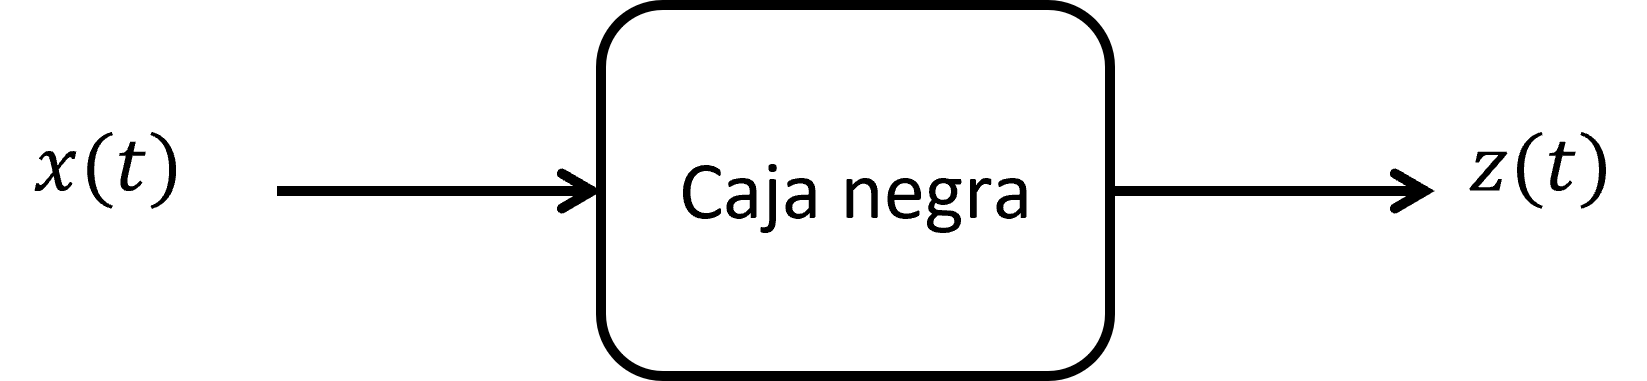
\includegraphics[scale=0.7]{Figuras/caja_negra.png}
        % \end{figure}
        
    \item Generar un ruido blanco de entrada. \emph{Nota:} La entrada debe ser una excitación persistente, es decir, la señal debe ser rica en un amplio espectro de frecuencias (suficientes armónicas).
    
    \item Medir $x[n]$ y $z[n]$.

    \item Realizar postprocesamiento a las señales de medición (detrend, resampling, etc.).
    
    \item Estimar $H_{true}(\omega) = G_{YU}(\omega)$ utilizando $H_1$ o $H_2$.\\

    \emph{Nota:} $|H_1(\omega)| \leq |H_{true}(\omega)| \leq |H_2(\omega)|$

    \item Calcular $\gamma_{ZX}^2$ y revisar la calidad de la estimación FRF.
    
        % \begin{figure}[H]
        %     \centering
        %     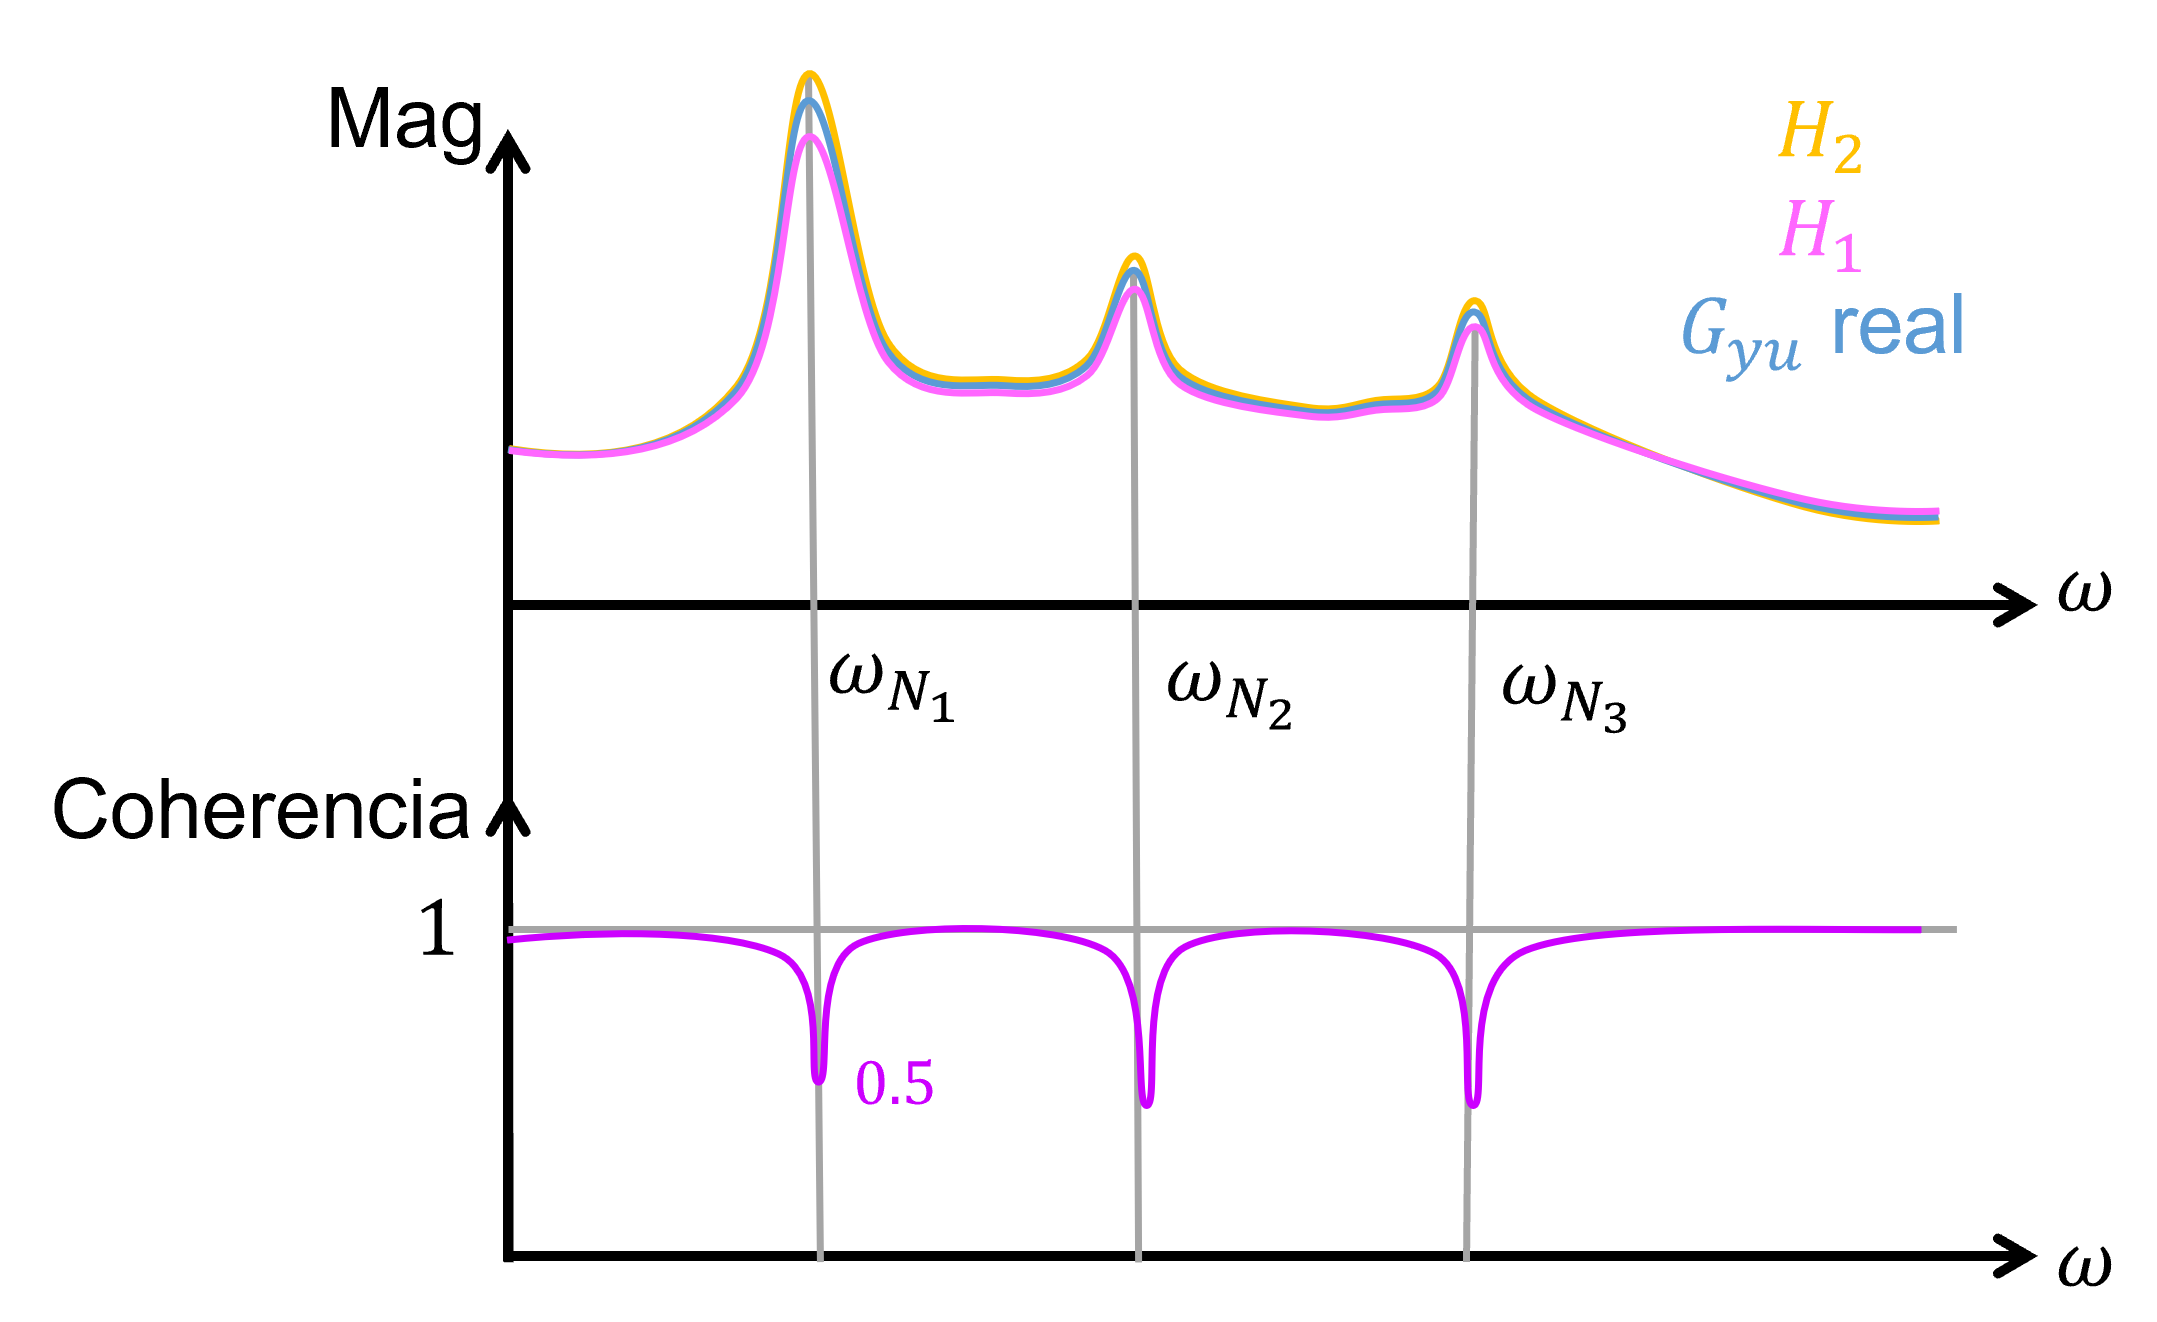
\includegraphics[scale=0.7]{Figuras/Gyu.png}
        % \end{figure}
        
\end{enumerate}

% En estricto rigor, $H_1$ y $H_2$ nos entregan una respuesta discretizada para valores de $\omega \in \{\omega_0,\omega_1,...,\omega_N\}$\\

En \emph{Matlab}, la función \texttt{tfestimate()} determina el FRF experimental con estimadores H1/H2, donde los periodogramas se determinan usando el método de Welch. Link:
\url{https://www.mathworks.com/help/signal/ref/tfestimate.html}.

% Otras alternativas son \texttt{etfe()} y \texttt{spa()}.

\subsection{Frecuencias y formas modales utilizando \emph{peak-picking}}

Referencia: \textcite[Sec. 18.6]{craig2006fundamentalsstructural}

Considere la EDM de un sistema MDOF:

\begin{equation}
    M \ddot{u} + C \dot{u} + K u = G p(t)
\end{equation}

\noindent donde $u(t) \in \mathbb{R}^n$ y $p(t) \in \mathbb{R}$ son los GLs y la excitación, respectivamente; $M \in \mathbb{R}^{n \times n}$, $C \in \mathbb{R}^{n \times n}$ y $K \in \mathbb{R}^{n \times n}$ son las matrices de masa, amortiguamiento y rigidez, respectivamente; $G \in \mathbb{R}^{n}$ es el vector de participación de la excitación $p(t)$ en la dinámica del sistema.

De la solución del problema de valores y vectores propios generalizados:

\begin{equation}
    K \phi = \lambda M \phi
\end{equation}

\noindent donde $\lambda_r = \omega_r^2$ y $\phi_r$ es el valor y vector propio del modo $r$. De este resultado podemos definir coordenadas modales  en notación matricial:

\begin{equation}
    u(t) = \Phi q(t)
\end{equation}

\noindent donde $\Phi = [\phi_1, \phi_2, \ldots,\phi_n]$ es la matriz de formas modales del sistema.

La relación entre coordenadas físicas y modales la podemos describir en notación indicial:

\begin{equation}\label{eq:coordmod}
    u_{s}(t) = \phi_{sr} q_r(t)    
\end{equation}

Asumiendo amortiguamiento proporcional, la EDM de la coordenada modal $q_r(t)$ se escribe:

\begin{equation}
    \ddot{q}_{r} + 2 \zeta_r \omega_r \dot{q}_{r}  + \omega_r^2 q_r = \underbrace{\phi_{kr} G_k}_{\gamma_r} p(t)
\end{equation}

Aplicando la transformada de Fourier, podemos calcular el FRF de la coordenada modal $q_r$ dada la entrada $p$:

\begin{equation}
    H_{q_{r} p}(\Omega) = \frac{\gamma_r}{(\omega_r^2 - \Omega^2) + j (2 \zeta_r \omega_r \Omega)}
\end{equation}

Volviendo a \eqref{eq:coordmod}, aplicando la transformada de Fourier:

\begin{align}
    U_{s}(\Omega) &= \phi_{sr} Q_r(\Omega) \\
                  &= \phi_{sr} H_{q_rp}(\Omega) P(\Omega) \\
                  &= H_{u_{s} p}(\Omega) P(\Omega)
\end{align}

Por lo tanto:

\begin{equation}
    H_{u_{s} p}(\Omega) = \frac{\gamma_r}{(\omega_r^2 - \Omega^2) + j (2 \zeta_r \omega_r \Omega)} \phi_{sr}
\end{equation}

Notar que cuando $\Omega = \omega_r$, el FRF tiene solo parte imaginaria:

\begin{equation}
    H_{u_{s} p}(\omega_r) = \frac{\gamma_r}{j (2 \zeta_r \omega_r^2)} \phi_{sr}
\end{equation}

Entonces, el peak ``r'' de la parte imaginaria de $H_{u_{s} p}$ es proporcional a la componente $\phi_{sr}$ de la forma modal $r$:

\begin{equation}
    \Im\left\{H_{u_{s} p}(\omega_r)\right\} \propto \phi_{sr}
\end{equation}

Podemos ocupar esta información para estimar las formas modales utilizando FRF experimentales:

\begin{figure}
    \centering
    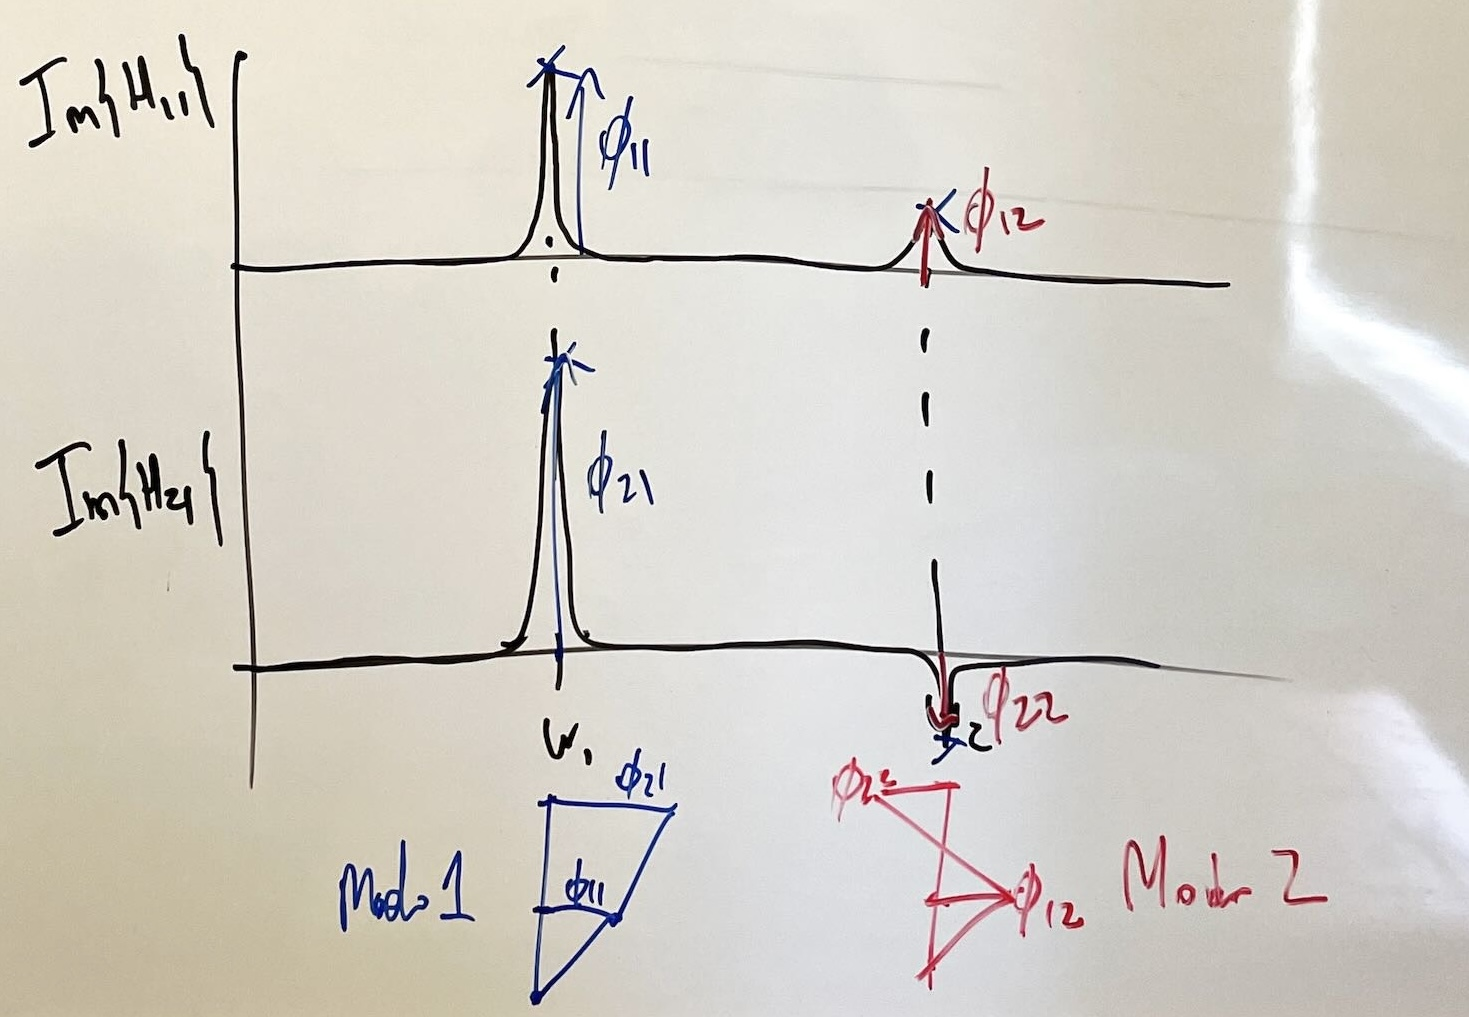
\includegraphics[width=6in]{Figuras/expmodeshapes.JPG}
    \caption{Estimación de formas modales}
\end{figure}

\subsection{Ajuste de modelos no paramétricos}

Métodos de estimación de parámetros \parencite[Cap. 7]{Ljung1998}:

\begin{itemize}
    \item Least squares (LS)
    \item Prediction-error methods (PEM)
    \item Maximum likelihood estimator (MLE)
    \item Instrumental Variable (IV)
\end{itemize}

System Identification Toolbox de Matlab. URL: \url{https://www.mathworks.com/help/ident/index.html}.

\section{Métodos de identificación \emph{ouput-only} }

En algunos casos no se conoce la entrada que actúa sobre el sistema estructural. En esas situaciones, la identificación del sistema se realiza solo a partir de las respuestas medidas (\emph{output-only}), como el desplazamiento, la velocidad o la aceleración. Estas respuestas se deben a excitaciones ambientales o de operación. A veces, el procedimiento se conoce como análisis modal operacional (\emph{operational modal analysis}, OMA).

\subsection{Frequency domain decomposition (FDD)}

El método de descomposición en el dominio de la frecuencia (FDD) permite aproximar las frecuencias y modos de vibrar a partir del cálculo de descomposición de valores singulares de la función de PSD \parencite{brincker2001modalidentification}. Los valores singulares se pueden utilizar para definir un sistema SDOF equivalente caracterizado por los mismos parámetros modales que el sistema MDOF que se está investigando.

% Sin embargo, la estimación de los modos de vibrar puede ser sesgada, debido a que la descomposición de valores singulares fuerza a que los vectores sean ortogonales. En caso de que los modos de vibrar sean ortogonales, la estimación no es sesgada.

Algoritmo:

\begin{enumerate}
    \item Medir respuesta multivariada del sistema $y[n] \in \mathbb{R}^{m \times 1}$. Esto quiere decir que se miden $m$ respuestas del sistema dinámico.
    \item Calcular auto PSD de respuesta $S_{yy}(\omega) \in \mathbb{R}^{m \times m}$ utilizando método de Welch.
    \item Descomponer $S_{yy}(\omega_i)$ utilizando SVD:

        \begin{equation}
            S_{yy}(\omega_i) = U_i \Sigma_i U_i^*, \qquad \forall i\in\{0,\ldots,N\}
        \end{equation}

    donde $U_i = [u_{i1}, u_{i2}, \cdots, u_{iN}]$.
    
    \item Graficar valores singular vs frecuencia, e identificar los peaks.
    \item En un peak asociado al modo $k$ (es decir, en frecuencia $\omega_k$), si no hay otros peaks cercanos, y es el peak dominante, entonces la primera columna de $U_k$ corresponde a la forma modal:

        \begin{equation}
            \varphi_k = u_{k1}
        \end{equation}
    
    y los valores singulares vecinos corresponden al auto PSD del sistema SDOF equivalente en coordenadas naturales.
    \item Utilizar indicador MAC (\emph{modal assurance criterion}) para decidir si la forma modal es adecuada. 
\end{enumerate}

\subsection{Enhanced Frequency Domain Decomposition (EFDD)}

El método \emph{Enhanced Frequency Domain Decomposition} (EFDD) es una extensión del método FDD que permite estimar no solo las frecuencias naturales, sino también las razones de amortiguamiento modales del sistema. Este procedimiento consiste en aislar los datos obtenidos mediante la descomposición en valores singulares (SVD) alrededor de un peak del espectro, y transformarlos al dominio del tiempo para obtener una función de correlación. A partir de esta función, se asume un comportamiento de un sistema de un solo grado de libertad (SDOF), lo que permite determinar con mayor precisión las frecuencias naturales y los amortiguamientos, de manera independiente de la resolución espectral y facilitando la identificación de modos cercanos en frecuencia.

%\subsection{Métodos de subespacio}

\subsection{Eigensystem Realization Algorithm (ERA)}

Referencia: \textcite{Juang1985}

Matlab: \texttt{era()}. URL: \url{https://www.mathworks.com/help/ident/ref/era.html}

\subsection{Natural Excitation Technique (NExT)}

El método \emph{Natural Excitation Technique} (NExT) se basa en que, cuando una estructura es excitada por una entrada de tipo ruido blanco, la función de correlación cruzada entre las respuestas medidas en dos puntos distintos es proporcional a la función de respuesta impulsiva (FRI) del sistema. Esto permite obtener la información dinámica de la estructura a partir únicamente de sus respuestas, sin necesidad de conocer la excitación aplicada.

%\subsection{Random Decrement Technique (RDT)}


\subsection{Stochastic Subspace Identification (SSI)}

Referencia: \textcite{vanoverschee2011subspaceidentification}

Clase de algoritmos que utilizan proyecciones (oblícuas) de subespacios y algebra lineal (factorización QR y SVD) para buscar la representación de variables de estado del sistema, $(A, B, C, D)$.

Alternativas para construir matriz Hankel: Data-Driven (SSI-DATA) y Covariance-Driven (SSI-COV).

% What it is: N4SID is the general name for the class of algorithms that use subspace projections (specifically, oblique projections) and linear algebra (like QR factorization and SVD) to find a system's state-space matrices (A, B, C, D).

% Application: It's a broad framework that can be used for both:

% Input-Output (Deterministic) ID: When you have measured both the input (e.g., shaker force) and the output (e.g., acceleration).

% Output-Only (Stochastic) ID: When you only have the output measurements and must assume the input is unknown white noise. When N4SID is used in this context, it is called Stochastic Subspace Identification (SSI).

% In short, SSI-DATA and SSI-COV are two specific types of N4SID adapted for the stochastic (output-only) case.

% 2. SSI-COV vs. SSI-DATA (The "Implementations")

% The fundamental difference between these two SSI methods is what data is used to build the main Block-Hankel matrix (the large matrix that organizes the system's past and future data).

% �� SSI-COV (Covariance-Driven)

% This is a two-step process that uses output covariances.

% Step 1: Calculate Covariances: The algorithm first computes the output covariance functions from the raw time-series data. This step essentially averages the data and acts as a form of data compression.

% Step 2: Build Hankel Matrix: It then constructs the Block-Hankel matrix using these calculated covariance values, not the raw data.

% Solve: The N4SID algorithm (SVD, etc.) is then applied to this covariance-based Hankel matrix to find the state-space model.

% Key Feature: It works with covariance functions. This can be computationally faster for extremely long datasets because the covariance matrix is much smaller than the raw data matrix.

% �� SSI-DATA (Data-Driven)

% This is a one-step process that works directly with the measurements.

% Step 1: Build Hankel Matrix: The algorithm constructs the Block-Hankel matrix directly from the raw time-series data.

% Solve: The N4SID algorithm (often involving an efficient QR factorization first, then SVD) is applied to this massive data matrix to find the state-space model.

% Key Feature: It works directly with raw time-series data. This avoids the intermediate step of calculating covariances (which can sometimes introduce bias) and is often considered more numerically robust.


% MAC: Modal Assurance Criterion

Función Matlab \texttt{n4sid()}. URL: \url{https://www.mathworks.com/help/ident/ref/n4sid.html}.